\documentclass[12pt]{article}
\usepackage[left=1in, right=1in, top=1in, bottom=1in, footnotesep=.25in]{geometry}
\usepackage{placeins}           % adds \FloatBarrier to keep floats in place
\usepackage[table]{xcolor}     % controls color of text, including headers
\usepackage{roboto}            % sans serif font for headers
\usepackage{crimson}           % serif font
\usepackage[T1]{fontenc}       % controls font enconding
\usepackage{sectsty}           % Allows for different fonts for header and body
\usepackage{lipsum}
\usepackage[hang,flushmargin]{footmisc} 
\usepackage{graphicx}          %%\includegraphics
\usepackage{pdfcomment}        % use \pdftooltip to add Alt-text to figure
\usepackage{tocloft}                 % format TOC, LOF, TOL
  %sectsty commands
  % all section headers use the same sans serif family - roboto
  \allsectionsfont{\sffamily\selectfont\roboto\mdseries\bfseries}
  % Set size and color of section header AL's H1
  \sectionfont{\roboto\LARGE\nohang\centering\textcolor[cmyk]{0.90, 0.54, 0.28, 0.12}}
    % Set size and color of subsection header AL's H2
  \subsectionfont{\fontsize{18pt}{20pt}\selectfont\roboto\nohang\centering\textcolor[cmyk]{0.90, 0.54, 0.28, 0.12}}
    % Set size and color of subsubsection header AL's H3
  \subsubsectionfont{\hspace{0pt}\nohang\fontsize{16pt}{18pt}\selectfont\roboto\raggedright\textcolor[cmyk]{0.50, 0.05, 0.0, 0.40}}
    % Set size and color of paragraph header AL's H4
    \paragraphfont{\fontsize{14pt}{16pt}\selectfont\robotocondensed\fontseries{bl}\selectfont\textcolor[cmyk]{0.50, 0.05, 0.0, 0.40}}
  
  %ditch section numbers
    \setcounter{secnumdepth}{0}
  
	% remove indent
    \parindent=0in
  
	% create new paragraph command to add new line after header
    \newcommand{\paragraphnewline}[1]{\paragraph{#1}\mbox{}\\}
	
  % footnote settings
    \renewcommand{\footnoterule}{\rule{2in}{.5pt}}
    \renewcommand{\thefootnote}{\arabic{footnote} }% space added as per Al's request
    
   %Ensure font in tables matches body font
    \makeatletter
      	\renewenvironment{table}%
  	    {\renewcommand{\familydefault}{\rmdefault}\selectfont
 	      \@float{table}}
  	    {\end@float}
    \makeatother



 % Set fonts in TOC, LOT, and LOF
 \renewcommand{\contentsname}{\hfill\sffamily\textcolor[cmyk]{0.90, 0.54, 0.28, 0.12}{Contents}\hfill} % set TOC title format
  \renewcommand{\cftaftertoctitle}{\hfill}         % centers TOC title
  \renewcommand{\listtablename}{\hfill\sffamily\textcolor[cmyk]{0.90, 0.54, 0.28, 0.12}{Tables}} % set LOT title format
  \renewcommand{\cftafterlottitle}{\hfill}         % center LOT title 
  \renewcommand{\listfigurename}{\hfill\sffamily\textcolor[cmyk]{0.90, 0.54, 0.28, 0.12}{Figures}} % set LOF title format
  \renewcommand{\cftafterloftitle}{\hfill}         % center LOF title
  \renewcommand\cftsecfont{\normalfont}            % set TOC section format
  \renewcommand\cftsubsecfont{\normalfont}         % set TOC subsection format
  \renewcommand\cftsubsubsecfont{\normalfont}      % set TOC subsubsection format
  \renewcommand\cftparafont{\normalfont}           % set TOC paragraph format
  \renewcommand\cftsecpagefont{\normalfont}        % set TOC section page number format
  \renewcommand\cftsubsecpagefont{\normalfont}     % set TOC subsection page number format
  \renewcommand\cftsubsubsecpagefont{\normalfont}  % set TOC subsubsection page number format
  \renewcommand\cftparapagefont{\normalfont}       % set TOC paragraph page number format
  \renewcommand\cfttabfont{\normalfont}            % set LOF font
  \renewcommand\cfttabpagefont{\normalfont}        % set LOF page number font
  \renewcommand\cftfigfont{\normalfont}            % set LOF font
  \renewcommand\cftfigpagefont{\normalfont}        % set LOF page number font
  
  % Set Tech Memo specific indent values for TOC
    % TOC indents
      \renewcommand{\cftsecindent}{0in}
      \renewcommand{\cftsubsecindent}{0.1701in}
      \renewcommand{\cftsubsubsecindent}{0.3418in}
    % LOF leaders and format
      \renewcommand{\cftfigpresnum}{Figure\ }
    \renewcommand{\cftfigaftersnum}{.}
    %LOT leaders and format
       \renewcommand{\cfttabpresnum}{Table\ }
       \renewcommand{\cfttabaftersnum}{.}
   
   % Correct spacing for LOF/T leaders 
    \newlength{\mylenf}
    \settowidth{\mylenf}{\cftfigpresnum\cftfigaftersnum}
    \setlength{\cftfignumwidth}{\dimexpr\mylenf+0.75em}
    \setlength{\cfttabnumwidth}{\dimexpr\mylenf+0.75em}

% Add dots between section titles and page numbers in TOC
    \renewcommand{\cftsecleader}{\cftdotfill{\cftdot}}
% Make dot spacing in TOC LOF/T match TM style
    \renewcommand{\cftsecdotsep}{1}
     \renewcommand{\cftsubsecdotsep}{0.4}
     \renewcommand{\cftsubsubsecdotsep}{0.4}
     \renewcommand{\cftfigdotsep}{0.5}
     \renewcommand{\cfttabdotsep}{0.5}

  %Set font in tables
    \makeatletter
	\renewenvironment{table}%
  	{\renewcommand{\familydefault}{\rmdefault}\selectfont
 	 \@float{table}}
  	{\end@float}
      \makeatother

%%The following sets up how the pdf displays links and functions in Acrobat.
\hypersetup{
    bookmarks    = true,        % show bookmarks bar?
    unicode      = false,       % non-Latin characters in Acrobat's bookmarks
    pdftoolbar   = true,        % show Acrobat's toolbar?
    pdfmenubar   = true,        % show Acrobat's menu?
    pdffitwindow = false,       % window fit to page when opened
    pdfstartview = {FitH},      % fits the width of the page to the window
    pdfnewwindow = true,        % links in new window
    colorlinks   = true,        % false: boxed links; true: colored links
    linkcolor    = black,        % color of internal links (change box color with linkbordercolor)
    citecolor    = black,       % color of links to bibliography
    filecolor    = black,        % color of file links
    urlcolor     = black         % color of external links
}

	
  % Create custom font title of document
  % note the use of:
  %% \textcolor in the title itself
  %%  \maketitle BEFORE resetting the \fontfamily
    \usepackage{xparse}
    \usepackage{xpatch}
       \NewDocumentCommand{\TitlePageFont}{}{%
        \sffamily\bfseries%
        \fontsize{22pt}{24pt}%
        \selectfont%
      }%
      \xpretocmd{\maketitle}{\TitlePageFont}{}{}
\title{\textcolor[cmyk]{1.00,0.83,0.41,0.36}{Example NWFSC Tech Memo Template}}
\author{Chantel Wetzel, Erin Steiner, Jason E. Jannot\\
\small{Al Brown will create title pages, thus the format of this page is not important.}}
 
\begin{document}
\maketitle
% Remove page number (not important if Al is doing title page but for OCD..)
\thispagestyle{empty}
\newpage
\normalfont % this sets the main font to crimson
\normalsize %% return the text to 12 point font - otherwise you end up with 22 point font from title page
\pagenumbering{roman}  %Set front matter (order: TOC, LOF, TOL, Executive Summary, Dedication, Acknowld) page numbers in lower roman numeral
\setcounter{page}{3}     % Start page number from iii as 1st 2 pages have no number
\tableofcontents
\newpage
\listoftables
\newpage
\listoffigures
\newpage
\section{Executive Summary}
This document acts as a template to create the format and style of a NWFSC Technical Memorandum using \LaTeX.\\
\\
\lipsum[1]
\lipsum[2]
\newpage
\section{Dedication}
Dedicated to all the excellent \LaTeX  users at NWFSC.
\newpage
\section{Acknowledgements}
We would like to thank Al Brown, Technical Editor for the NWFSC for his help, patience, and fortitude during this process.
\newpage
\pagenumbering{arabic}
\setcounter{page}{1}
\thispagestyle{empty}	
\section{Document Layout}
The layout in this document serves as an example of the order of parts for the front matter, main text, and back matter.
\section{Page Layout}
\subsection{Page Numbering}
The first page of the introduction should not have a page number; however, the arabic page number 1 should appear in the TOC. To accomplish this, simply add the following commands at the end of the Acknowledgements, before the Introduction section.\\
\\
\texttt{\textbackslash pagenumbering\{arabic\}\\
	\textbackslash setcounter\{page\}\{1\}\\
	\textbackslash thispagestyle\{empty\}\\
}

\subsection{Fonts}
\FloatBarrier
\begin{table}[h]
\caption{Font specifications for NWFSC NOAA Technical Memorandums}
\begin{center}
\begin{tabular}{llrll}
%\begin{tabular}
\textbf{Text} & \textbf{Typeface} & \textbf{Size (pt.)} & \textbf{Color (cmyk)} & \textbf{Align}\\
\hline
Title & {\selectfont\roboto\fontseries{b} roboto bold} & 22 & 1.00,0.83,0.41,0.36 & right\\
Subtitle & {\selectfont\roboto\normalfont roboto regular} & 18 & 1.00,0.83,0.41,0.36 & right\\
Header 1 & {\selectfont\roboto\fontseries{b} roboto bold} & 20 & 0.94,0.54,0.28,0.12 & center\\
Header 2 & {\selectfont\roboto\fontseries{b} roboto bold} & 18 & 0.94,0.54,0.28,0.12 & center\\
Header 3 & {\selectfont\roboto\fontseries{b} roboto bold} & 16 & 0.50,0.05,0.00,0.41 & left\\
Header 4 & {\selectfont\robotocondensed\fontseries{bl} roboto light condensed bold} & 14 & 0.50,0.05,0.00,0.41 & left\\
Header 5 & {\selectfont\robotocondensed\fontseries{l}\itshape roboto light condensed italic} & 14 & 0.50,0.05,0.00,0.41 & left\\
Body & crimson & 12 & black & left \\
\hline
\end{tabular}
\end{center}
\end{table}
\FloatBarrier
\subsection{Margins and Spacing}
Page margins should be 1 inch all around.  Spacing between each paragraph should be 12 point.
\subsection{Footnotes}
Footnotes in tables are generally frowned upon.  However, if you must, table footnotes for NOAA Technical Memorandum use lowercase letter(s) as the footnote indicator. The footnote\footnote{Text footnotes are in arabic numerals with a space between note and script, in 10 point font.} at the bottom of this page discusses how to set up footnotes in the body. Footnote numbering restarts from 1 in each appendix.\\
\section{Figures and Tables}
\subsection{Tables}
Tables have no vertical lines and no shading.  Table and caption font is crimson, the same as the body text. Font size within tables can be 9 - 11 point, but font size must be the same for all tables. Captions are 11 point font left aligned, the width of the page with a 0.3 inch hanging indent on the second and subsequent lines, and appear above the table.  The table is centered 0.125 inches below the caption.  More table specifications can be found in the NWFSC Style Guide\footnote{https://homeport.northwestscience.fisheries.noaa.gov/outreach\_media/Publishing/Style\_Guide/sg\_format\_tabfig.cfm}.
\subsection{Figures}
Colors palettes used in figures can be found on the NWFSC website\footnote{https://homeport.northwestscience.fisheries.noaa.gov/outreach\_media/Publishing/tmpr\_colors.cfm}.  Caption font is crimson, the same as the body text. Captions are 11 point font left aligned, the width of the page with a 0.3 inch hanging indent on the second and subsequent lines, and appear below the figure.  The figure is centered 0.125 inches above the caption.  More figure specifications can be found in the NWFSC Style Guide\footnote{https://homeport.northwestscience.fisheries.noaa.gov/outreach\_media/Publishing/Style\_Guide/sg\_format\_tabfig.cfm}.

\begin{figure}[!h]
\centering
\caption[Demo Alt-text]{This is meant to demo the use of \texttt{\textbackslash pdftooltip} to add Alt-Text to a figure.}
\label{fig:diamprice5k}
 \pdftooltip{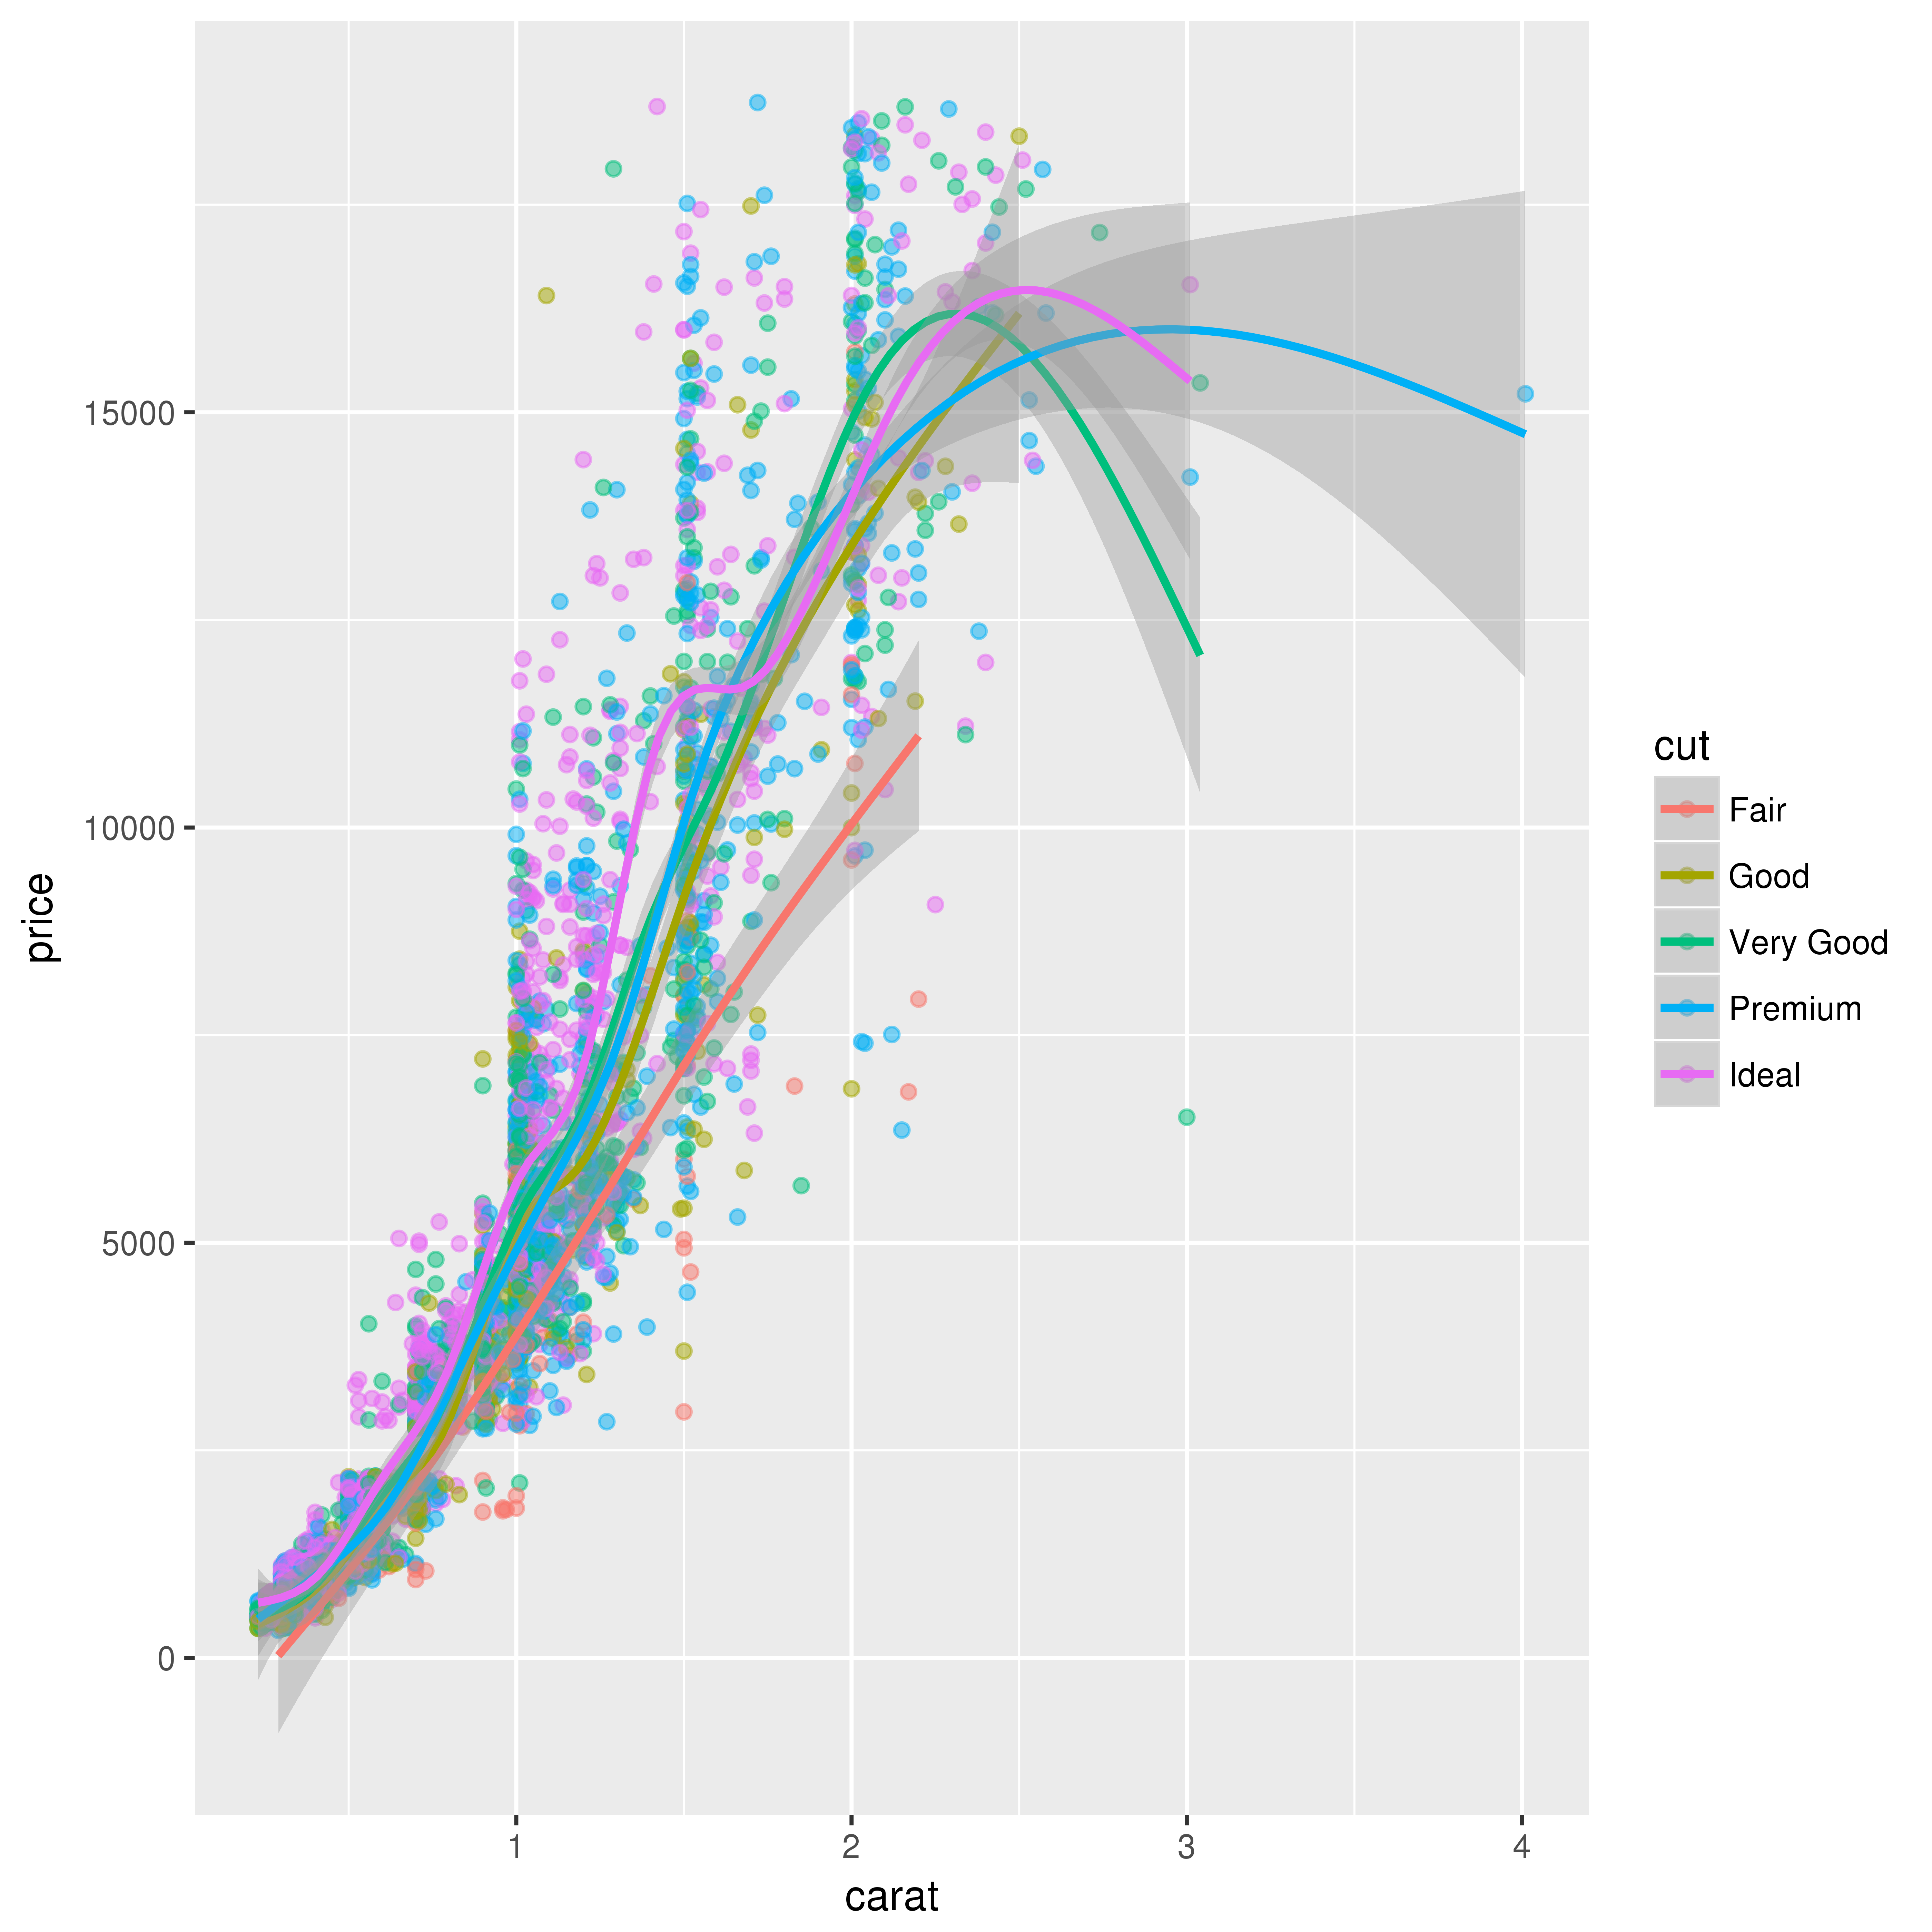
\includegraphics[scale=0.75]{diamprice5k.png}}{Here is a plot of the prices of 5,000 round cut diamonds.}
\end{figure}

\section{Cross-References and Hyperlinks}
Cross-references and hyperlinks are not colored -- they're just black. So all TOC, LOT, and LOF entries and in-line references to tables or figures should be black. Hyperlinks are also black. In the body text, they're underlined and footnoted. In the footnote, the URL is written out in full but is black and not underlined. 

\section{More Examples}
For anything not addressed above, please see the NWFSC Style Guide or email Al Brown, NWFSC Technical Editor.
The remainder of this document is simply meant to show how to format various headers not captured above and to add more entries into the TOC, LOT, and LOF.
\subsection{Subsection Header}
\lipsum[5]
\subsubsection{Subsubsection Header}
\lipsum[3]
\begin{figure}[h]
\caption{Another figure}
\centering lmnop
\end{figure}

\lipsum[6]

\paragraphnewline{Paragraph Header}
\lipsum[7]

\begin{table}[h]
\caption{Some other table}
\centering qrstuv
\end{table}

\begin{table}[h]
\caption{Some table}
\centering abc
\end{table}

\lipsum[4]

\section{References}
put your references here.
\newpage
\appendix
\section{Example appendix}

\end{document}